\begin{flushright} {\tiny {\color{gray} pair\_crouzeixraviart.tex}} \end{flushright}
%~~~~~~~~~~~~~~~~~~~~~~~~~~~~~~~~~~~~~~~~~~~~~~~~~~~~~~~~~~~~~~~~~~~~~~~~~~~~~~~~~~~~~~~~~~~~~~~~~~

Since the $P_2\times P_{-1}$ pair is not LBB stable \cite[p179]{reddybook2}, 
(see also table 3.13-1 of \textcite{grsa})
it is enhanced by a cubic bubble and is therefore called $P_2^+\times P_{-1}$. 

This element was first introduced in \cite{crra73}.
It is a seven-node triangle (in 2D) with quadratic velocity shape 
functions enhanced by a cubic bubble function and discontinuous linear interpolation for 
the pressure field \cite{cuss86}. 
This element is LBB stable and no additional stabilization techniques are required\cite{elsw}.
The '+' in its name stands for the bubble while the '-' stands for the discontinuous
character of the pressure field: once again, it is $P_1$ over the element, but discontinuous
across element edges.
It is the element used in the MILAMIN code \cite{daks08}.

\begin{remark}
Cuvelier \etal, 1986 \cite{cuss86} recommend a 6-point or 7-point quadrature rule for this element.
\end{remark}

\begin{remark}
Segal \cite{segal} explains 
for output purposes (printing, plotting etc.) the discontinuous pressures are averaged 
in vertices for all the adjoining elements. See also Fig. 7.3 of \cite{cuss86}.
\end{remark}

\begin{remark}
The simplest Crouzeix-Raviart element is the non-conforming linear triangle 
with constant pressure \cite{cuss86}, see Section~\ref{ss:p1ncp0}.
\end{remark}

It is worth noting that this element has more degrees of freedom  than the 
Taylor-Hood element for the same order of accuracy. However, since the 
bubble can be eliminated, one can design a modified version of this element.
\todo[inline]{Check Cuvelier book chapter 8 for modified element}

\begin{remark}
I have once asked the (main) author of MILAMIN why he chose this element, for 
example over the $P_2\times P_1$. His answer is as follows:
"Elements with continuous pressure  are incapable of converging in the Linf 
norm for mechanical problems exhibiting pressure jumps such as the inclusion-host setup. 
During my MSc and PhD I was focusing on sharp heterogeneities, so this is why I decided 
to choose $P_2^+\times P_{-1}$. 
You will see that it is also easy to invert the pressure mass matrix for such elements, 
which is really useful (both for the augmentation and preconditioning)."
\end{remark}

This element is used by Poliakov and Podlachikov \cite{popo92} to study the deformation of 
the surface above a rising diapir. Note that they actually use a 
``13 point integration formula (Hughes 1987) for calculation of the stiffness matrix was 
used in order to conserve detailed information from the marker field in the coarse FEM mesh''. 
It is also used in \cite{anmp15} in the context of a new free-surface stabilization scheme. 
It is the element used in LaCoDe \cite{demh19}.
It is mentioned in Section~6.2 in \textcite{bobf08} (2008).
It is compared to the $P_2\times P_1$ element for the Navier-Stokes equations in 
\textcite{krba05} (2005).

\begin{center}
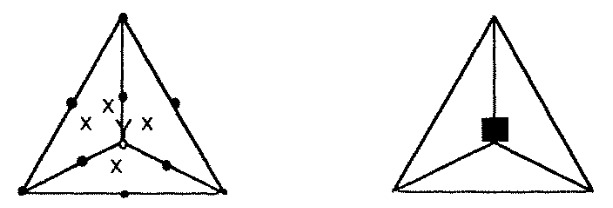
\includegraphics[width=6cm]{images/pair_cr/cr}\\
{\captionfont Taken from \textcite{begt92} (1992).}
\end{center}

The 3D version of this element is presented in \textcite{begt92} (1992). 
In their Table III we find the following node coordinates and basis functions:
\[
\begin{array}{lll}
\text{\# node} & \text{coordinates} & \text{basis function} \\
1  & (0,0,0) & \bN_1(r,s,t)=(1-r-s-t) -\frac12 (\bN_5+\bN_7+\bN_8)-\frac13(\bN_{11}+\bN_{12}+\bN_{13})-\bN_{15}/4 \\ 
2  & (1,0,0) & \bN_2(r,s,t)=r-\frac12(\bN_5+\bN_6+\bN_9)    -\frac13(\bN_{11}+\bN_{12}+\bN_{14}) -\bN_{15}/4 \\
3  & (0,1,0) & \bN_3(r,s,t)=s-\frac12(\bN_6+\bN_7+\bN_{10}) -\frac13(\bN_{11}+\bN_{13}+\bN_{14}) -\bN_{15}/4 \\
4  & (0,0,1) & \bN_4(r,s,t)=t-\frac12(\bN_8+\bN_9+\bN_{10}) -\frac13(\bN_{12}+\bN_{13}+\bN_{14}) -\bN_{15}/4 \\
5  & (\frac12,0,0)             &  \bN_5(r,s,t)=4(1-r-s-t)r-\frac49(\bN_{11}+\bN_{12})-\bN_{15}/4  \\
6  & (\frac12,\frac12,0)       &  \bN_6(r,s,t)=4rs-\frac49(\bN_{11}+\bN_{14})-\bN_{15}/4  \\
7  & (0,\frac12,0)             &  \bN_7(r,s,t)=4(1-r-s-t)s-\frac49(\bN_{11}+\bN_{13})-\bN_{15}/4  \\
8  & (0,0,\frac12)             &  \bN_8(r,s,t)=4(1-r-s-t)t-\frac49(\bN_{12}+\bN_{13})-\bN_{15}/4  \\
9  & (\frac12,0,\frac12)       &  \bN_9(r,s,t)=4rt-\frac49(\bN_{12}+\bN_{14})-\bN_{15}/4  \\
10 & (0,\frac12,\frac12)       &  \bN_{10}(r,s,t)= 4st-\frac49(\bN_{13}+\bN_{14})-\bN_{15}/4 \\
11 & (\frac13,\frac13,0)       &  \bN_{11}(r,s,t)= 27(1-r-s-t)rs-\frac{108}{256}\bN_{15} \\
12 & (\frac13,0,\frac13)       &  \bN_{12}(r,s,t)= 27(1-r-s-t)rt-\frac{108}{256}\bN_{15} \\
13 & (0,\frac13,\frac13)       &  \bN_{13}(r,s,t)= 27(1-r-s-t)st-\frac{108}{256}\bN_{15} \\
14 & (\frac13,\frac13,\frac13) &  \bN_{14}(r,s,t)= 27rst-\frac{108}{256}\bN_{15} \\
15 & (\frac14,\frac14,\frac14) &  \bN_{15}(r,s,t)= 256(1-r-s-t)rst \\
\end{array}
\]

We have
\begin{eqnarray}
\bN_1+\bN_2+\bN_3+\bN_4 
&=& (1-r-s-t) -\frac12 (\bN_5+\bN_7+\bN_8)-\frac13(\bN_{11}+\bN_{12}+\bN_{13})-\bN_{15}/4 \nn\\
&+& r-\frac12(\bN_5+\bN_6+\bN_9)    -\frac13(\bN_{11}+\bN_{12}+\bN_{14}) -\bN_{15}/4 \\
&+& s-\frac12(\bN_6+\bN_7+\bN_{10}) -\frac13(\bN_{11}+\bN_{13}+\bN_{14}) -\bN_{15}/4 \\
&+& t-\frac12(\bN_8+\bN_9+\bN_{10}) -\frac13(\bN_{12}+\bN_{13}+\bN_{14}) -\bN_{15}/4 \\
&=& 1 -\frac12(1+1)\bN_5 -\frac12(1+1)\bN_6 -\frac12(1+1)\bN_7 -\frac12(1+1)\bN_8 -\frac12(1+1)\bN_9 -\frac12(1+1)\bN_{10}    \nn\\
&&  -\frac13(1+1+1)\bN_{11} -\frac13(1+1+1)\bN_{12} -\frac13(1+1+1)\bN_{13} -\frac13(1+1+1)\bN_{14} 
-\frac{1}{4}(1+1+1+1)\bN_{15} \nn\\
&=& 1 -\bN_5 -\bN_6 -\bN_7 -\bN_8 -\bN_{9} -\bN_{10}
      -\bN_{11} -\bN_{12} -\bN_{13} -\bN_{14} -\bN_{15} 
\end{eqnarray}
So in the end
\[
\sum_{i=1}^{15} \bN_i = (\bN_1+\bN_2+\bN_3+\bN_4)  + \sum_{i=5}^{15} \bN_i = 0
\]

